\documentclass[unknownkeysallowed,xcolor=table]{beamer}
 
\usepackage[T2A,T1]{fontenc}
\usepackage[utf8]{inputenc}
\usepackage[english,russian]{babel}
\usepackage{amsmath}
\usepackage{listings}
\usepackage{url}
\usepackage{textcomp}
\usepackage{multirow}
\usepackage{tikz}

\setbeamertemplate{navigation symbols}{}

\usetikzlibrary{arrows,shapes,decorations.markings,positioning}

\tikzstyle{entity} = [rectangle, minimum width=0.5cm, minimum height=3cm, text width=2cm, text centered, draw=black, fill=blue!20]
\tikzstyle{file} = [rectangle, minimum height=1.5cm, text width=1cm, text centered, draw=black, fill=orange!30]
\tikzstyle{tool} = [rectangle, rounded corners, minimum width=0.5cm, text width=1cm, text centered, draw=black, fill=green!20]

\tikzstyle{vecArrow} = [thick, decoration={markings,mark=at position
   1 with {\arrow[semithick]{open triangle 60}}},
   double distance=1.4pt, shorten >= 5.5pt,
   preaction = {decorate},
   postaction = {draw,line width=1.4pt, white,shorten >= 4.5pt}]
\tikzstyle{innerWhite} = [semithick, white,line width=1.4pt, shorten >= 4.5pt]

\newcommand{\textapprox}{\raisebox{0.5ex}{\texttildelow}}

\newcommand{\rarr}{$\rightarrow$}
 
\colorlet{mygreen}{green!60!blue}
\colorlet{mymauve}{red!60!blue}
\definecolor{light-gray}{gray}{0.9}

\lstset{
      basicstyle=\ttfamily\small,
      commentstyle=\color{mygreen},
      keywordstyle=\color{blue},
      numberstyle=\tiny\color{blue},
      stringstyle=\color{mymauve},
      numbers=left,
      stepnumber=1,
      columns=fullflexible,
      breaklines=true,
      postbreak=\mbox{\textcolor{red}{\ensuremath{\hookrightarrow}\space}},
      literate={~} {\textapprox}{1},
      language={[11]C++}
}

\lstnewenvironment{cmdline}
  {\lstset{
      basicstyle=\ttfamily\scriptsize,
      keywordstyle=\color{blue},
      backgroundcolor=\color{light-gray},
      language={bash}
  }}
  {}

\lstnewenvironment{cmdlinelarge}
  {\lstset{
      basicstyle=\ttfamily\small,
      keywordstyle=\color{blue},
      backgroundcolor=\color{light-gray},
      language={bash}
  }}
  {}

\makeatletter
\newcommand{\srcmediumsize}{\@setfontsize{\srcmediumsize}{7pt}{7pt}}
\makeatother

\makeatletter
\newcommand{\srcbigsize}{\@setfontsize{\srcbigsize}{8pt}{8pt}}
\makeatother

\makeatletter
\newcommand{\srcsize}{\@setfontsize{\srcsize}{6pt}{6pt}}
\makeatother

\makeatletter
\newcommand{\srcsmallsize}{\@setfontsize{\srcsmallsize}{5pt}{5pt}}
\makeatother

\title[C++]
{Программирование на языке C++}
 
\subtitle{Вводный курс}
 
\author[А.~Б.~Морозов]
{
  \texorpdfstring{Александр Морозов\newline\href{mailto:gelu.speculum@gmail.com}{gelu.speculum@gmail.com}}
  {Александр Морозов}
}
  
\date[ITMO 2022]
{ИТМО, весенний семестр 2022}
 
\logo{%
  \makebox[0.97\paperwidth]{%
    
\includegraphics[align=c,width=2cm,keepaspectratio]{itmo_logo.png}
    \hfill
    
\includegraphics[align=c,width=1.5cm,keepaspectratio]{itiviti_logo.png}
  }
}

\AtBeginSection[]
{
  \begin{frame}
    \frametitle{Содержание}
    \tableofcontents[currentsection]
  \end{frame}
}

\begin{document}
 
\frame{\titlepage}

%-------------------------------------------------
\section{Вступление}

\begin{frame}{О чём этот курс?}
  \begin{itemize}
    \item Основные элементы языка C++ \vspace{3em}
    \item Некоторые инструменты для разработки программ на C++ \vspace{3em}
    \item Базовые навыки программирования
  \end{itemize}
\end{frame}

\begin{frame}{Почему C++?}
  \begin{itemize}
    \item Язык сочетает черты низкоуровневого и высокоуровневого \vspace{1em}
    \item Позволяет как использовать сложные абстракции, так и прибегать к низкоуровневым оптимизациям и ручному управлению ресурсами \vspace{1em}
    \item Zero overhead abstractions \vspace{1em}
    \item Значительно более высокоуровневый, чем C, но в то же время может быть настолько же эффективным \vspace{1em}
    \item Один из самых распространенных прикладных языков
  \end{itemize}
\end{frame}

\begin{frame}{Место C++ в современном мире}
  \begin{itemize}
    \item Графические оболочки (MS Windows UI, Aqua, KDE)
    \item Офисные пакеты (MS Office, OpenOffice)
    \item Графические редакторы и среды 3D моделирования (Photoshop, Maya)
    \item Компьютерные игры (CryEngine, Frostbite, Gamebryo, id Tech 4-, Source, Unreal Engine)
    \item CAD (Autodesk, Catia, FreeCAD)
    \item Браузеры и Javascript движки (Chrome, Firefox, V8, SpiderMonkey)
    \item Базы данных (MongoDB, частично MariaDB, MS SQL, Oracle, SAP DB, ScyllaDB)
    \item Системы информационного поиска, интернет поисковики (Google, Яндекс)
    \item Финтех (Bloomberg, Morgan Stanley, Itiviti)
  \end{itemize}
\end{frame}

\begin{frame}{Что не так с Java?}
  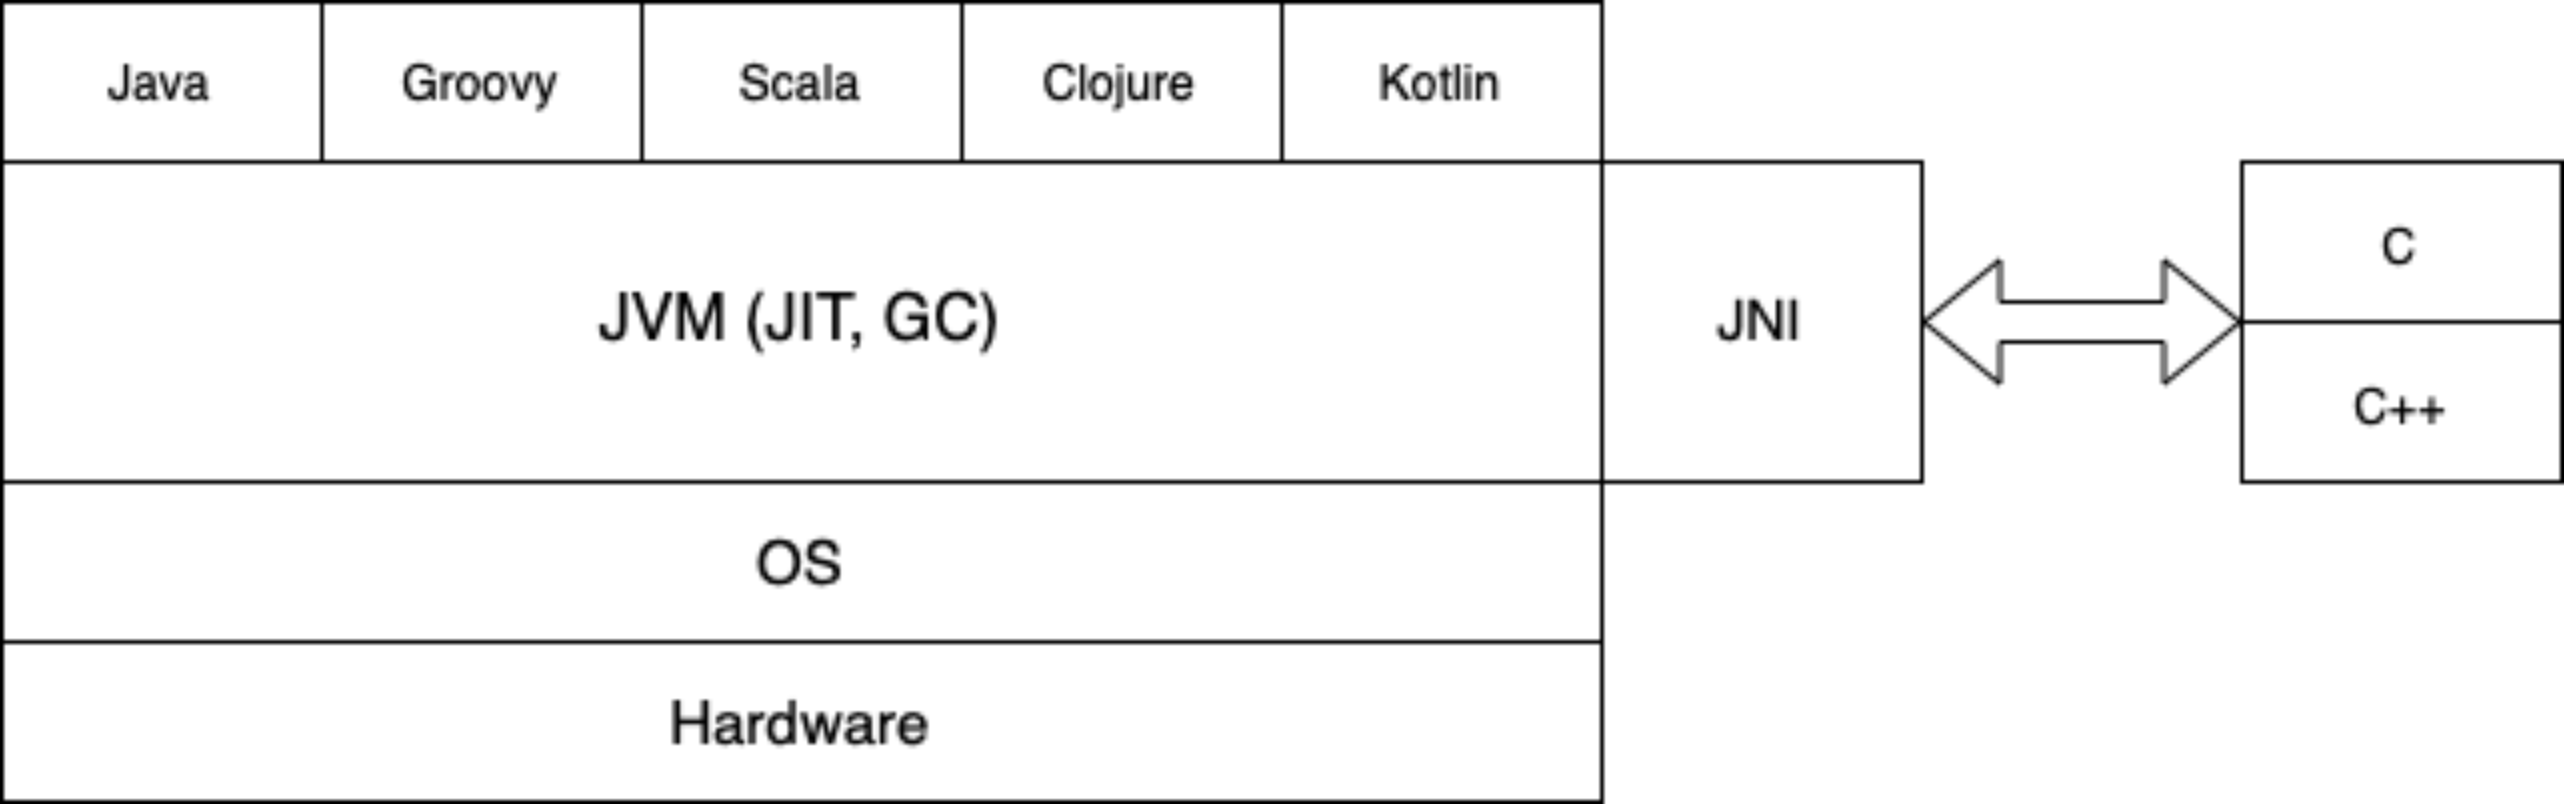
\includegraphics[align=c,width=10cm,keepaspectratio]{images/JVM.png}
\end{frame}

\begin{frame}{Что не так с другими компилируемыми языками?}
\end{frame}

\begin{frame}{Интероперабельность C++ с другими языками}
  \begin{itemize}
    \item с JVM -- так себе, JNI \vspace{1em}
    \item с .NET -- Managed/Unmanaged C++, есть подводные камни \vspace{1em}
    \item с различными интерпретируемыми -- ? \vspace{1em}
    \item с различными компилируемыми -- FFI (обычно, C интерфейс)
  \end{itemize}
\end{frame}

\begin{frame}{Что не так с C++?}
  \begin{itemize}
    \item катастрофически сложен \vspace{1em}
    \item иногда слишком примитивен \vspace{1em}
    \item иногда недостаточно современен \vspace{1em}
    \item эволюция путём добавления элементов и механизмов
  \end{itemize}
\end{frame}

\begin{frame}[fragile]{Сложности грамматики C++}
  \begin{lstlisting}
    // variables 'x', 'y', 'z'
    int(x), y, *const z;

    // expression '(int(x)), (y), (new int))'
    int(x), y, new int;

    // ??
    B b(A());
  \end{lstlisting}
\end{frame}

\begin{frame}[fragile]{Тонкости и нюансы в C++ важны}
  \begin{lstlisting}
    int a; // type of 'a' = int
    decltype(a) b; // type of 'b' = int
    decltype((a)) c; // type of 'c' = int &
  \end{lstlisting}
\end{frame}

\begin{frame}[fragile]{В C тоже были весёлые моменты}
  \begin{lstlisting}
    int n = sizeof(0)["abcdef"];
    // n == ??
  \end{lstlisting}
\end{frame}

\begin{frame}[fragile]{Эволюционные сложности C++}
  \begin{lstlisting}
    static vs static vs static

    struct vs class vs typename
  \end{lstlisting}
\end{frame}

\begin{frame}{Сложности правил языка}
  \begin{itemize}
    \item 9 различных видов инициализации переменных \vspace{2em}
    \item 21 правило упорядочивания исполнения \vspace{2em}
    \item 13 правил выбора лучшего кандидата при перегрузке функций \vspace{2em}
    \item и ещё больше веселья в шаблонах
  \end{itemize}
\end{frame}

\begin{frame}[fragile]{Ещё больше веселья с инициализацией в C++20}
  \begin{lstlisting}
    struct A
    {
      int && r;
    };

    A a1{7}; // lifetime is extended
    A a2(7); // lifetime is NOT extended
  \end{lstlisting}
\end{frame}

\begin{frame}{Формат курса}
  \begin{itemize}
    \item Лекции \vspace{1em}
    \item Небольшие примеры-иллюстрации к лекциям \vspace{1em}
    \item Задачи по мотивам примеров \vspace{1em}
    \item Большие задачи \vspace{1em}
    \item Соревнование по скорости для 2-й большой задачи \vspace{1em}
    \item Сдача задач через code review на github.com \vspace{1em}
    \item Коллоквиум в середине семестра \vspace{1em}
    \item Экзамен
  \end{itemize}
\end{frame}

\begin{frame}{Некоторая литература}
  \begin{itemize}
    \item Bjarne Stroustrup: Programming: Principles and Practice Using C++, 2014\\Программирование Принципы и практика использования С++
    \item Bjarne Stroustrup: The C++ Programming Language (4th edition), 2013
    \item Bjarne Stroustrup: The Design and Evolution of C++, 1994\\Дизайн и эволюция C++
    \item Stanley Lippman: C++ Primer (5th Edition), 2012\\Язык программирования C++. Базовый курс
    \item Herb Sutter: Exceptional C++, 1999; More Exceptional C++, 2001\\Решение сложных задач на С++
    \item и другие: Meyers, Josuttis, Alexandrescu, Vandevoorde
  \end{itemize}
\end{frame}

%-------------------------------------------------
\section{История}

\begin{frame}{Предшественники C++}
  \begin{itemize}
    \item Simula: объектно-ориентированный язык, 1965 \vspace{3em}
    \item C: эффективный процедурный язык, 1972
  \end{itemize}
\end{frame}

\begin{frame}{Появление C++: цели создателя}
  Бьярне Страуструп занимался моделированием распределенных аспектов операционных систем и ему нужен был язык:
  \begin{itemize}
    \item ООП
    \item пользовательские абстракции
    \item сильная типизация
    \item эффективность
    \item отсутствие ``необоснованной стоимости'' возможностей
    \item простота реализации (использование уже существующих инструментов)
    \item отсутствие излишних ограничений на стиль программирования
  \end{itemize}
\end{frame}

\begin{frame}{Краткая история C++}
  1979 - C with classes (расширение языка C классами, наследованием, более сильной типизацией, встраиваемыми функциями).

  1983 - C++ (перегрузка функций и операторов, виртуальные функции, ссылки, типобезопасное управление памятью).

  1985 - The C++ Programming Language (первое описание языка).

  1989 - C++ 2.0 (множественное наследование, абстрактные классы, статические члены классов).

  1990 - The Annotated C++ Reference Manual (шаблоны, исключения, пространства имен).

  1992 - STL (обобщенная реализация различных структур данных и типовых алгоритмов).

  1998 - C++98, первый ISO стандарт языка.
\end{frame}

\begin{frame}{Краткая история C++, продолжение}
  1999 - Boost.

  2003 - C++03, второй ISO стандарт, незначительные изменения.

  2011 - С++11, новый стандарт, большие изменения и модернизация.

  2013 - 4-е издание The C++ Programming Language.

  2014 - C++14, дальнейшее развитие нового стандарта.

  2017 - C++17, текущий \emph{устоявшийся} стандарт языка.

  2020 - C++20, текущий \emph{опубликованный} стандарт языка.
\end{frame}

\begin{frame}{Классификация языков программирования}
  \begin{itemize}
    \item Компилируемые / интерпретируемые \vspace{1em}
    \item Императивные / декларативные \vspace{1em}
    \item Поддержка различных парадигм: ООП, функциональные, логические \vspace{1em}
    \item Статическая типизация / динамическая типизация \vspace{1em}
    \item Сильная типизация / слабая типизация \vspace{1em}
    \item Энергичные / ленивые
  \end{itemize}
\end{frame}

%-------------------------------------------------
\section{Абстрактная вычислительная машина}

\begin{frame}{Нижний уровень языка}
  \begin{itemize}
    \item целые числа и операции над ними в рамках двоичного представления
    \item дробные числа имеют определённую точность и диапазон
    \item типы данных вместо битов и байтов в памяти
    \item линейная непрерывная память
    \item по умолчанию -- последовательное исполнение (в рамках observable behaviour)
    \item начиная с C++11 модель памяти учитывает параллельное исполнение
    \item управление параллельным исполнением в стандартной библиотеке
    \item исключения заданы высокоуровневым поведением
  \end{itemize}
\end{frame}

\begin{frame}{Ниже этих абстракций}
  \begin{itemize}
    \item Особенности конкретной архитектуры, например, big-ending vs little-endian; битность процессора
    \item Целые и дробные числа представляются по-разному
    \item Много уровней памяти: регистры, кеш нескольких уровней, RAM
    \item Реальный и защищенный режим
    \item Виртуальная память
    \item Прерывания, системные вызовы, переключение контекста
    \item Параллелизм: внутри ядра процессора, между несколькими ядрами, между процессорами; разные гарантии синхронизации на разных архитектурах
    \item Инструкции различной сложности: RISC, CISC, векторные инструкции, сопроцессоры (“математический”, GPU)
  \end{itemize}
\end{frame}

\begin{frame}{Гарантии языка и undefined behaviour}
  \begin{itemize}
    \item Некоторые вещи язык гарантирует - вне зависимости от платформы, компилятора и иных внешних факторов. Например, \lstinline{sizeof(int) <= sizeof(long)}.
    \item \emph{Observable behaviour}: компилятор может менять программу, если её внешнее поведение не меняется.
    \item \emph{Implementation defined behaviour}: поведение программы может различаться в зависимости от реализации компилятора (но это должно быть задокументировано).
    \item \emph{Unspecified behaviour}: поведение зависит от реализации, но это не требуется документировать; каждый возможный вариант поведение должен быть корректным.
    \item \emph{Undefined behaviour}: стандарт не накладывает никаких ограничений на поведение в этом случае.
  \end{itemize}
\end{frame}

%-------------------------------------------------
\section{Трансляция программ на языке C++}

\begin{frame}[fragile]{Структура программ на языке C++}
  \begin{itemize}
    \item набор текстовых файлов \vspace{1em}
    \item соглашение: заголовочные файлы и файлы кода \vspace{1em}
    \item соглашение: расширения \textbf{.h} и \textbf{.cpp} \vspace{1em}
    \item набор определений \vspace{1em}
    \item одно определение функции main
  \end{itemize}
\end{frame}

\begin{frame}{3 этапа трансляции C++}
  \begin{figure}
    \begin{tikzpicture}[node distance=2.5cm, auto,>=latex', thick]

      \node (src) [file] {\tiny .cpp};
      \node (cpp) [tool, below of=src] {\hspace{0pt}\tiny Препроцессор};
      \node (tmp) [file, below of=cpp] {\tiny tmp};
      \node (c++) [tool, right of=tmp] {\hspace{0pt}\tiny Компилятор};
      \node (asm) [file, above of=c++] {\tiny .s};
      \node (as) [tool, above of=asm] {\hspace{0pt}\tiny Ассемблер};
      \node (obj) [file, right of=as] {\tiny .o};
      \node (linker) [tool, below of=obj] {\hspace{0pt}\tiny Компоновщик};
      \node (exe) [file, below of=linker] {\hspace{0pt}\tiny executable};
      \node (lib) [file, right of=linker] {\hspace{0pt}\tiny Библиотеки};

      \draw[vecArrow] (src) -- (cpp);
      \draw[innerWhite] (src) -- (cpp);

      \draw[vecArrow] (cpp) -- (tmp);
      \draw[innerWhite] (cpp) -- (tmp);

      \draw[vecArrow] (tmp) -- (c++);
      \draw[innerWhite] (tmp) -- (c++);

      \draw[vecArrow] (c++) -- (asm);
      \draw[innerWhite] (c++) -- (asm);

      \draw[vecArrow] (asm) -- (as);
      \draw[innerWhite] (asm) -- (as);

      \draw[vecArrow] (as) -- (obj);
      \draw[innerWhite] (as) -- (obj);

      \draw[vecArrow] (obj) -- (linker);
      \draw[innerWhite] (obj) -- (linker);

      \draw[vecArrow] (linker) -- (exe);
      \draw[innerWhite] (linker) -- (exe);

      \draw[vecArrow] (lib) -- (linker);
      \draw[innerWhite] (lib) -- (linker);

    \end{tikzpicture}
  \end{figure}
\end{frame}

\begin{frame}[fragile]{Трансляция C++ на примере gcc}
  Трансляция программы из одного файла:
  \begin{cmdlinelarge}
    g++ -std=c++17 -o prog prog.cpp
  \end{cmdlinelarge}
  Результат препроцессора:
  \begin{cmdlinelarge}
    g++ -std=c++17 -E prog.cpp
  \end{cmdlinelarge}
  Ассемблерный код:
  \begin{cmdlinelarge}
    g++ -std=c++17 -S prog.cpp
  \end{cmdlinelarge}
  Объектный файл:
  \begin{cmdlinelarge}
    g++ -std=c++17 -c prog.cpp
  \end{cmdlinelarge}
  Дизассемблирование:
  \begin{cmdlinelarge}
    objdump -dS prog
  \end{cmdlinelarge}
\end{frame}

\begin{frame}{Объектные файлы}
  Объектные файлы обычно состоят из различных секций. Например: заголовок, секция кода, секция данных, отладочная информация.

  Сущности ссылаются по именам, адреса в памяти не назначены.

  Mangling: имена сущностей из текста программы не всегда могут быть перенесены в имена в объектном файле. Для C обычно соответствие точное (хотя некоторые реализации добавляют к имени дополнительную информацию). В C++ структура имен более сложная и они приводятся к уникальным строковым именам по определенному алгоритму (зависит от реализации).\\
  Например, имя \lstinline{Space::Outer::Inner::code} может быть преобразовано в \lstinline{_ZN5Space5Outer5Inner4codeE}.
\end{frame}

\begin{frame}{Online компиляторы}
  \begin{itemize}
    \item Coliru  \href{https://coliru.stacked-crooked.com/}{https://coliru.stacked-crooked.com/} \vspace{2em}
    \item Wandbox  \href{https://wandbox.org/}{https://wandbox.org/} \vspace{2em}
    \item Godbolt  \href{https://godbolt.org/}{https://godbolt.org/} \vspace{2em}
    \item CPP Insights \href{https://cppinsights.io/}{https://cppinsights.io/} \vspace{2em}
    \item Quick Bench \href{https://quick-bench.com/}{https://quick-bench.com/}
  \end{itemize}
\end{frame}

%-------------------------------------------------
\section{Организационные вопросы}

\begin{frame}{План лекций}
  \begin{enumerate}
    \item Вводная
    \item Основы языка
    \item Препроцессор, единицы трансляции, макросы
    \item Сложные типы данных
    \item Специальные методы классов
    \item Работа с памятью
    \item Предварительный обзор поздних тем
    \item Коллекции и итераторы
    \item \emph{Коллоквиум}
    \item Пространства имён
    \item Перегрузка функций
    \item ООП
    \item Шаблоны
    \item Исключения и безопасность
  \end{enumerate}
\end{frame}

\begin{frame}{Практические задания}
  \begin{itemize}
    \item Маленькие задачи -- 4 варианта по мотивам примера из лекции \vspace{2em}
    \item Большие задачи
      \begin{itemize}
        \item 4 набора по 3 задачи \vspace{1em}
        \item наборы в целом сбалансированы
      \end{itemize}
  \end{itemize}
\end{frame}

\begin{frame}{Дедлайны}
  \begin{itemize}
    \item Маленькие задачи: март -- апрель \vspace{2em}
    \item Большие задачи: апрель -- начало июня \vspace{2em}
    \item Финальный дедлайн -- экзамен, в первой половине сессии
  \end{itemize}
\end{frame}

\begin{frame}{Работа над задачей}
  \begin{itemize}
    \item 1-й дедлайн -- дедлайн оформления \vspace{1em}
    \item 2-й дедлайн -- дедлайн приёмки \vspace{1em}
    \item 2 недели между двумя дедлайнами \vspace{1em}
    \item code review -- несколько итераций \vspace{1em}
    \item работа \textbf{строго индивидуальная} \vspace{1em}
    \item по одной из больших задач возможно собеседование \vspace{1em}
    \item 14 ``поздних'' дней
  \end{itemize}
\end{frame}

\begin{frame}{Соревнование по скорости}
  \begin{itemize}
    \item параллельно с процессом ревью \vspace{1em}
    \item 2 прогона, можно внести изменения после 1-го \vspace{1em}
    \item места распределяются по перцентилям \vspace{1em}
    \item множитель оценки $1 \dotso 3$
  \end{itemize}
\end{frame}

\begin{frame}{Оценивание задач}
  \begin{itemize}
    \item базовая стоимость маленьких задач -- 5-12 баллов \vspace{1em}
    \item базовая стоимость больших задач -- 15-40 баллов \vspace{1em}
    \item суммарная базовая стоимость 3 больших задач -- 80 баллов \vspace{1em}
    \item штрафные баллы: число ревью, число существенных замечаний, число ``пушей'' на Github \vspace{1em}
    \item соревнование по скорости -- коэффициент масштабирования оценки за задачу
  \end{itemize}
\end{frame}

\begin{frame}{Теоретическая аттестация}
  \begin{itemize}
    \item Коллоквиум в середине семестра
    \item Экзамен в конце
      \begin{itemize}
        \item блиц
        \item основная часть
      \end{itemize}
  \end{itemize}
\end{frame}

\begin{frame}{Итоговая аттестация}
  \begin{itemize}
    \item Финальная оценка = оценка за экзамен
    \item Блиц
      \begin{itemize}
        \item провал = \textbf{F}
        \item успех = \textbf{E} или переход к основной части экзамена
      \end{itemize}
    \item Основная часть экзамена = оценка от \textbf{F} до \textbf{A}
    \item Успешно сданный коллоквиум заменяет блиц
    \item Допуск к экзамену -- порог баллов за задачи
      \begin{itemize}
        \item 70 баллов для блиц части
        \item 90 баллов для основной части
      \end{itemize}
    \item Автомат
      \begin{itemize}
        \item 125 баллов = \textbf{B}
        \item 150 баллов = \textbf{A}
      \end{itemize}
  \end{itemize}
\end{frame}

\begin{frame}{Иные источники баллов}
  \begin{itemize}
    \item улучшения тестов к задачам \vspace{2em}
    \item оформление конспекта
  \end{itemize}
\end{frame}

\begin{frame}{Сложности курса}
  \begin{itemize}
    \item язык сложный \vspace{1em}
    \item материала много \vspace{1em}
    \item студенты недооценивают сложность \vspace{1em}
    \item студенты переоценивают свои силы \vspace{1em}
    \item язык не похож на Java
  \end{itemize}
\end{frame}

\end{document}
